\section{Problem Formulation}
\label{sec:notation}

In this section, we provide background on uncertain graph, motivate the basic privacy attack, and formulate the uncertain graph anonymization problem. 

\vspace{-2.5pt}
\subsection{Uncertain Graph}
\vspace{-2.5pt}
An uncertain graph $\mathcal{G}=(V,E,\mathit{p})$, is defined over a set of nodes $V$, a set of edges $E$, and a set of probabilities $\mathit{p}$ of edge existence. Following the literature~\cite{Potamias_K_2010,Zhao_Detecting_2014,Colbourn_Colbourn_1987}, we assume possible-worlds semantics, and we consider the edge probabilities independent~\footnote{We leave the conditional probability model as a future
extension.}. An uncertain graph $\mathcal{G}=(V,E,\mathit{p})$ essentially represents a probability distribution over all of the certain graphs $G$ in the forms of which the uncertain graph may actually exist. 
The probability of observing any possible world $G_i=(V,E_{G_i})$ is    
\begin{equation*}
    Pr[G_i]=\prod_{e \in E_{G_i}} {\mathit{p}(e)} \prod_{e \in E \setminus E_{G_i}} 1-\mathit{p}(e)
\end{equation*}




\subsection{Privacy Attack}
\label{sec:AMPC}
\vspace{-5pt}
\begin{figure}[!htb]
  \vspace{-10pt}
    \subfigure[Social Trust Network]{\label{fig:socialNetwork}
      \begin{minipage}[l]{0.46\columnwidth}
        \centering
        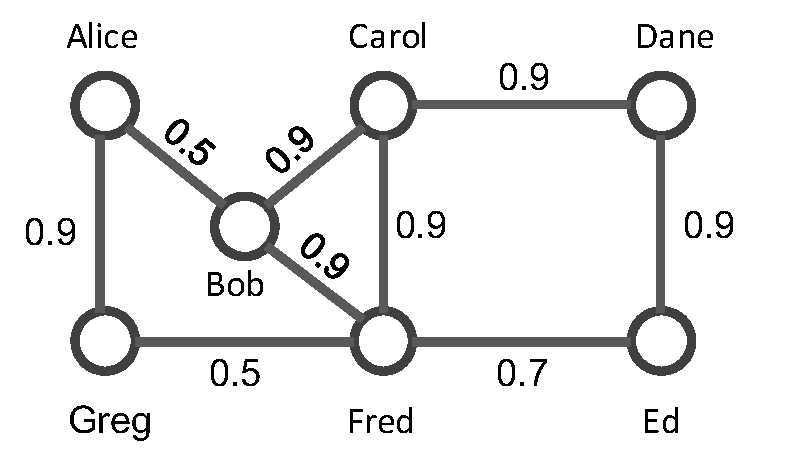
\includegraphics[height=2.7cm]{ill/example_source.pdf}
      \end{minipage}
      }
    \subfigure[The naive anonymization]{\label{fig:b2bNetwork}
      \begin{minipage}[l]{0.46\columnwidth}
        \centering
        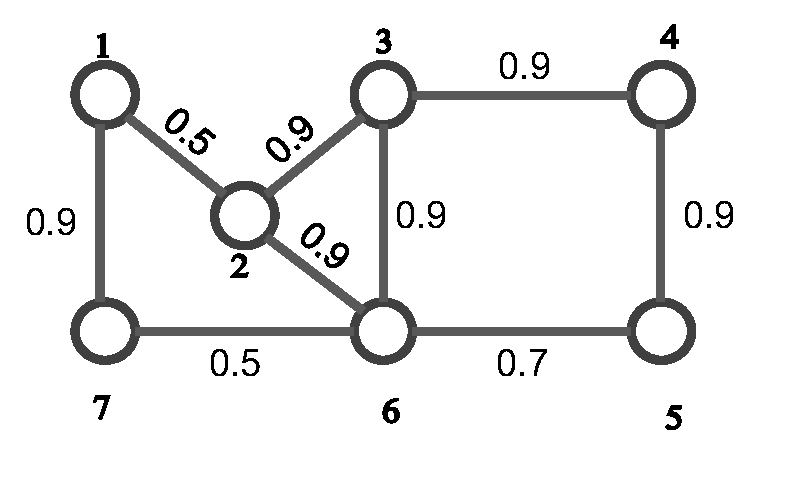
\includegraphics[height=2.7cm]{ill/example_output.pdf}
      \end{minipage}
      }
    \vspace{-7pt}
    \caption{The Structural Re-Identification Issue.}
    \label{fig:privacyAttack}
    \vspace{-7pt}
\end{figure} 
Obviously, simply removing the identities of the nodes before publishing the uncertain graph data does not guarantee privacy.  The structure of the uncertain graph itself, and in its basic form the degree of the nodes, can be revealing the identities of individuals. 
In practice the adversary may have access to external information about the entities in the graphs. This information may be obtained by the adversary's malicious actions. For example, for the uncertain graph in Figure~\ref{fig:privacyAttack}, the adversary might know that ``Freq has three or more \textbf{trust} neighbors“. Such information allows adversary to narrow down the set of candidates in the sanitized graphs. For example, the statement partially re-identify Freq as $\lbrace 2,3,6 \rbrace$ with \textbf{probabilities} respectively. Different to the deterministic scenario,  there are varying posterior probabilities over candidate nodes $\lbrace 2,3,6 \rbrace$. The node is vulnerable to the re-identification risk. Entity Re-identification (ER) can lead to additional disclosures. In this paper, we focus on the ER attack as this attack is one of the most serious privacy problem. 


\subsection{Privacy Notion}
\label{sec:privacyNotion}
To resist re-identification attacks, we adopt the $(k,\epsilon)$-obf, an syntactic privacy notion,
% introduced by Boldi {\etal}~\cite{Boldi_Injecting_2012},
 where $k \ge 1$ is a desired level of obfuscation  and $\epsilon \ge 0$ is a tolerance parameter. 

\textsc{Obfuscation Parameter}~~Similar to $k-$anonymity, $k-$obf requires blending every entity with other fuzzy matching entities. While, the level of obfuscation is quantified as the entropy over posterior probabilities over fuzzy matching ones. It lower bounds the entropy of the distribution by $\log_{2} k$. 

\textsc{Tolerance parameter}~~As for the tolerance parameter $\epsilon$, it serves for the following purpose. There might be extreme unique nodes, e.g., Trump in a Twitter network, whose obfuscation is almost impossible. Thus, Bonchi {\etal} introduce a tolerance parameter $\epsilon$, which allows skipping up to $\epsilon * |V|$ nodes and makes the privacy goal more practical. 

Though it is initially used to measure the privacy guarantee provided by an uncertain graph for the  deterministic graph, the stochastic nature makes it a good fit in the uncertain scenario. 
% The formal definition is,
% \theoremstyle{definition}
% \begin{definition}
% 	\textbf{\boldmath{$(k,\epsilon)$}-obf \cite{Boldi_Injecting_2012}}
%     Let $P$ be a vertex property (i.e., vertex degree in our work), $k \geq 1$ be a desired level of anonymity, and $\epsilon >0 $ be a tolerance parameter. 
%     An sanitized uncertain graph $\tilde{\mathcal{G}}$ is said to $k$-obfuscate a given vertex $v \in \mathcal{G}$ w.r.t $P$ if the entropy $H()$ of the distribution $Y_{P(v)}$ over the nodes 
%     of $\tilde{\mathcal{G}}$ is greater than or equals to $\log_{2}{k}$:
%     \begin{equation*}
%         H(Y_{P(v)}) \geq \log_{2}{k}.
%     \label{obfCon}
%     \end{equation*}
% The uncertain graph $\tilde{\mathcal{G}}$
% is $(k,\epsilon)$-obf w.r.t property $P$ 
% if it $k$-obfuscates at least $(1-\epsilon)|V|$ nodes in $\mathcal{G}$. 
% \label{def:obf}
% \end{definition} 
\subsection{Utility Loss Metric: Reliability Discrepancy}

As a fundamental property, connectivity plays an important role in graph mining tasks such as nearest neighbor locating and graph clustering. The connectivity model is shown to yield a better graph representation than the degree sequence mode ~\cite{Liu_Privacy_2009}.  Connectivity discrepancy was proven to be a proper utility-loss metric in deterministic graph anonymization. 

In the uncertain scenario, the concept of reliability is used to generalize connectivity. It captures the probability that two given nodes are reachable over all possible worlds. Similarly, we  use reliability discrepancy as the utility-loss metric in the uncertain scenario. 

\begin{definition}
    \textbf{Two-Terminal Reliability~\cite{Colbourn_Colbourn_1987}}~~Given an uncertain graph $\mathcal{G}$, and two distinct nodes $u$ and $v$  $\in~V$, the reliability of $(u,v)$ is defined as:
        \begin{equation*}
                R_{u,v}(\mathcal{G})= \sum_{G \in W(\mathcal{G})}  \mathcal{I}_{G}(u,v) Pr[G] 
        \end{equation*}
    where $\mathcal{I}_{G}(u,v)$ is 1 iff $u$ and $v$ are contained in a connected component in $G$, and 0 otherwise.   
    \label{d:reliability}
\end{definition}



\theoremstyle{definition}
\begin{definition}
    \textbf{Reliability Discrepancy (RD)}
    The reliability discrepancy of graph $\tilde{\mathcal{G}}=(V,E, \tilde{\mathit{p}})$, 
    denoted as $\Delta(\tilde{\mathcal{G}})$, 
    w.r.t. the original graph  $\mathcal{G}$ is 
    defined as the sum of the two-terminal reliability discrepancy over all node pairs $(u,v) \in V_\mathcal{G}$.
    \begin{equation*}
        \Delta(\tilde{\mathcal{G}})=\sum_{(u,v) \in V_\mathcal{G} }|R_{u,v}(\mathcal{G})-R_{u,v}(\tilde{\mathcal{G}})|
    \end{equation*}
\end{definition}

\subsection{Problem Statement}
Given the above foundation, we can now formulate our goal.  
\vspace{-15pt}
\begin{problem}
     Given an uncertain graph $\mathcal{G}$ and desired anonymization parameters $k$ and $\epsilon$, 
     the objective is to find a  $(k,\epsilon)$-obf uncertain graph $\tilde{\mathcal{G}}$
     with the minimal utility loss, as 
     \vspace{-5pt}
     \begin{equation*}
             \begin{aligned}
                 & \argmin_{\tilde{
                \mathcal{G}}} & & \Delta(\tilde{\mathcal{G}}) \\
                &  \text{Subject to} & &\tilde{\mathcal{G}} \text{~is~} (k,\epsilon)-obf
            \end{aligned}
     \end{equation*}
     \label{prob:unobf}
\end{problem}
% add one paragraph to ....